
% This is the EASV CS21 4th Semester IOT Exam project report.
% Group name is


% Preamble
\documentclass[12pt, a4, utf8]{report}        % here is the document's type which is {article}.
\title{title}                       % the title of this document.
\author{Fei Gu}
\date{\today}

% Packages
\usepackage{amsmath}
\usepackage{graphicx}


% Document
\begin{document}        % the ducument start here
    \maketitle
    \tableofcontents


    \section{Problem statement}\label{sec:problem-statement}
    % Which problem for a human is it solving and why is it important


    \section{Illustration of network architecture}\label{sec:illustration-of-network-architecture}
    % Use draw.io make a architecture, remember to name the protocols and the hardwares.


    \paragraph{}
    Following the problem statement, we have to design the architecture base on three different terminal using three ESP32 MCU.


    \paragraph{}
    The first terminal which connect to the all sensor component will try to get the data.
    And then when the data value reach to a limit then send a message to MQTT server by Wi-Fi connection, at the
    same time send the data to "Blynk.console" to show the data.


    \paragrapg{}
    The MQTT server will subscribe the topic where


    \section{Illustration of the hardware setup}\label{sec:illustration-of-the-hardware-setup}
    % Use fritzing or just use circuiTikZ make the circuit layout\pm

    \subsection{esp32No1 Sensor}\label{subsec:esp32no1-sensor}

    \begin{figure}[h]
        \caption{ESP32 no.1 connect to sensors}
        \centering
        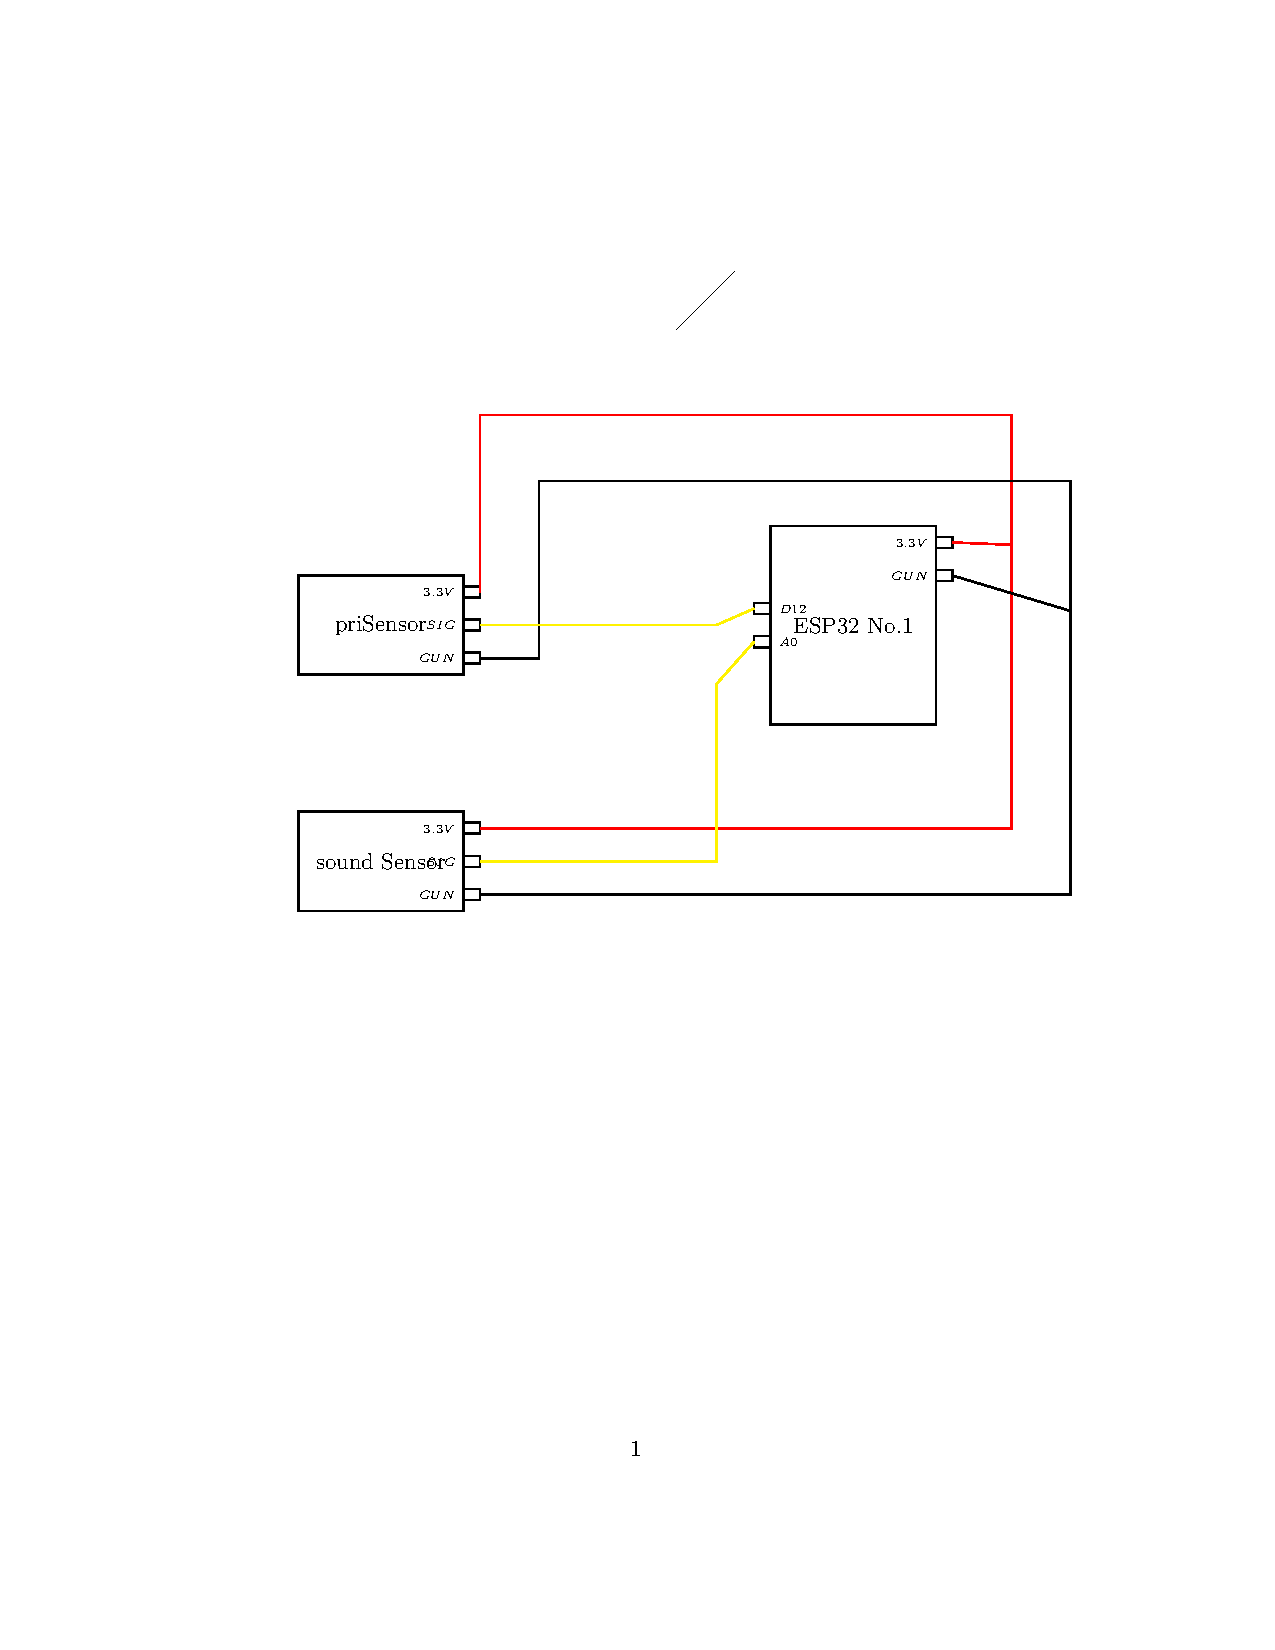
\includegraphics[width=0.5\textwidth]{../out/ESP32_No1_connect_Sensor}
        \label{fig:figure2}
    \end{figure}


    \subsection{esp32No2 Sensor}\label{subsec:esp32no2-sensor}

        \begin{figure}[h]
        \caption{ESP32 no.2 connect to buzzer and LED-display}\label{fig:figure3}
        \centering
        \includegraphics[width=0.5\textwidth]{../out/fullCircuitLayOut}

    \end{figure}

    \subsection{esp32Cam }\label{subsec:esp32cam}

    \paragraph{}
    This part is the connection about the Esp32 Camera can be flash under the develop mode.

    \begin{figure}[h]

        \caption{ESP32 CAM}\label{fig:figure4}
        \centering
        \includegraphics[width=0.5\textwidth]{../out/ESP32Cam_connect_TypeCAdapter}

    \end{figure}



    \bibliography{report}
    \bibliographystyle{plain}

\end{document}
